\documentclass{article}
\usepackage[utf8]{inputenc}
\usepackage{hyperref}
\usepackage{amsmath}
\usepackage{graphicx}
\usepackage{amssymb}
\title{CSC412 Notes Week 4}
\author{Jerry Zheng}
\date{April 2021}
\hypersetup{
    colorlinks=true,
    linkcolor=blue,
    filecolor=magenta,      
    urlcolor=blue,
    pdftitle={Sharelatex Example},
    bookmarks=true,
    pdfpagemode=FullScreen,
}

\begin{document}

\maketitle
\section{Exact Inference}
Lets say we have a distribution. $P(x, y)$
If we want to perform inference on it we would use $P(y|x) = \frac{P(x,y)}{\sum_{y}p(x,y)}$
However, there may be a set of variables in our model P that isn't apart of x or y.

$$x = \text{The observed evidence}$$
$$y = \text{The unobserved variable we want to infer} $$
$$r = X - {x, y} $$

Where $r$ is a set of random variables neither apart of the query nor the evidence.

$$p(y | x) = \frac{p(y, x)}{p(x)}$$

each of the distributions we need to compute can be computed by marginalizing over the other variables.

$$p(y, x) = \sum_{r}p(y, x, r)$$

However, naively marginalizing over all unobserved variables requires a number of computations exponential in the number of random variables, (N), in our model.

\section{Variable Elimination}
To compute this efficiently we will use the Variable Elimination Algorithm.\\
\\
It's an exact inference algorithm, meaning it will calculate exactly $p(y|x)$.\\
\\
It's also general, meaning it can be used on many different kinds of graphical models.\\
\\
It's complexity depends of the conditional independence of our model.\\
\\
It's intuitively done with dynamic programming.

\subsection{Chain Example}
$$ A \rightarrow B \rightarrow C \rightarrow D $$

To find P(D), we have the variables

$$y = \{D\}$$
$$x = \{\}$$
$$r = \{A, B, C\} $$

\begin{align*} 
P(y) &= \sum_{r} p(y, r) \\ 
\Rightarrow P(D) &= \sum_{A, B, C}p(A, B, C, D) \\ 
& = \sum_A \sum_B \sum_C p(A)p(B | A) p(C | B) p(D | C) \\
\end{align*}

This is exponential in the number of variables $\mathbf O(k^n)$ (k is the number of states per variable). But, reordering the joint distribution

$$ P(D) = \sum_C p(D | C) \sum_B p(C | B) \sum_A p(A)p(B | A) $$

we can begin to simplify

\begin{align*} 
P(D) &= \sum_C p(D | C) \sum_b p(C | B) \sum_A p(A)p(B | A) \\
&= \sum_C p(D | C) \sum_B p(C | B) \tau (B) \\
&= \sum_C p(D | C) \tau (C) \\
\end{align*}

So, by using dynamic programming to do the computation in reverse, we do inference over the joint distribution represented by the chain without generating it explicitly!\\
We have reduced the running time to $\mathbf{O(nk^2)}$!

\subsection{bigger example}

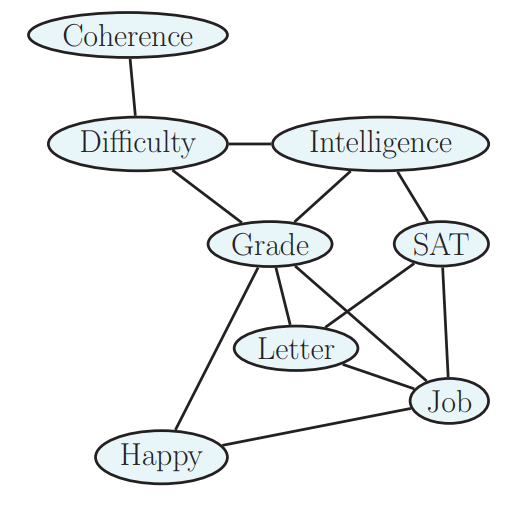
\includegraphics[scale=0.7]{Screenshot_12.png}\\
The joint distribution of our CS student graph is given by

$$P (C, D, I, G, S, L, J, H) = P (C)P (D|C)P (I)P (G|I, D)P (S|I)P (L|G)P (J|L, S)P (H|G, J)$$

with factors

$$P(C, D, I, G, S, L, J, H) = {\psi_C(C), \psi_D(C, D), \psi_I(I), \psi_G(G, I, D),  \psi_S(S, I), \psi_L(L, G), \psi_J(J, L, S), \psi_H(H, G, J)} $$
 (the textbook uses an undirected graph, not too important as variable elimination can be done all the same.)\\
 (an explanation of $\psi$ will be given in week 5's notes)\\
\\
To compute p(J = 1), we could calculate all possible assignments\\
$$p(J) = \sum_{L} \sum_{S} \sum_{ G} \sum_{ H} \sum_{ I} \sum_{D} \sum_{C}p(C, D, I, G, S, L, J, H)$$
But we can do better with variable elimination. Where we push sums inside products.\\

\begin{align*}
p(J) &= \sum_{L,S,G,H,I,D,C} p(C, D, I, G, S, L, J, H)\\
&= \sum_{L,S,G,H,I,D,C}\psi_C(C)\psi_D(D, C)\psi_I(I)\psi_G(G, I, D)\psi_S(S, I)\psi_L(L, G) \times \psi_J(J, L, S)\psi_H(H, G, J)\\
&= \sum_{L,S}\psi_J(J, L, S)
\sum_{G}\psi_L(L, G)
\sum_{H}\psi_H(H, G, J)
\sum_{I}\psi_S(S, I)\psi_I(I)
\times \sum_{D}\psi_G(G, I, D)
\sum_{C}\psi_C(C)\psi_D(D, C)
\end{align*}
from here we will marginalize out each variable individually to get a new factor at each step.\\
We do it in the order C, D, I, H, G, S, L to get P(J)\\

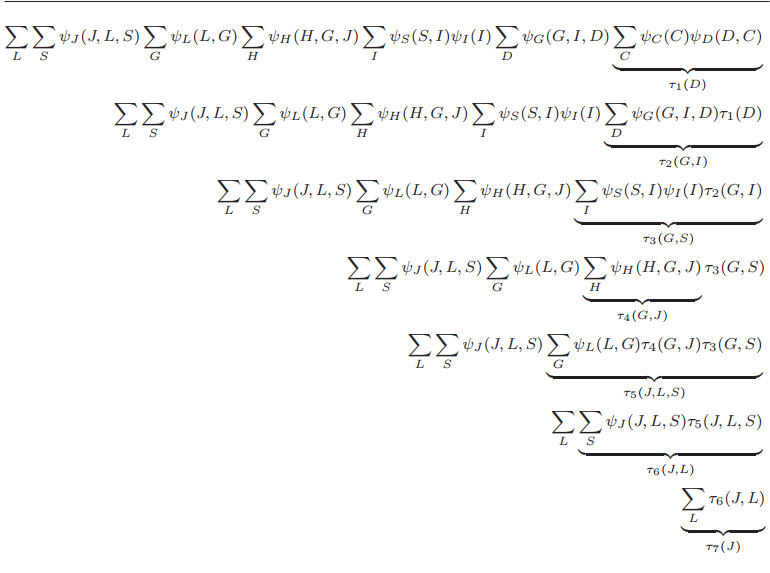
\includegraphics[scale=0.6]{Screenshot_13.png}

\end{document}
